% 07. kapitulua - Scrumban agentikoa
% Izenak: metodoa = Scrumban agentikoa (ingelesez: Agentic Scrumban); gainbegirale-agentea = scrumban-agentea.
% Lehen zirriborroa: izenaren jatorria, Scrum eta Kanban zer diren, zergatik nahastu lantalde hibrido batean
% (Scrum inplementaziorako, Kanban exekuziorako), eta metodoaren elementuen begirada orokorra.
% Garatzeko (TODO atalean): zereginaren egoera-makina, eskalatze-protokoloa, trazabilitatea.
% Irudiak: Pictures/07/ (goiburu hutsa header_07.pdf.xoj; bi begizten irudia marrazteko: 7.bi_begiztak.xoj)

Aurreko kapituluetan taldea osatu dugu, zereginak idazten ikasi dugu, biltegia antolatu dugu, proiektu-taula eskuz kudeatu dugu eta, azkenik, kodetzeko agenteak ezagutu ditugu.
Falta dena da hori guztia lotzen duen \textbf{lan egiteko modua}: nork erabakitzen du zer egin, nork egiten du, nork egiaztatzen du eta zer erritmotan.
Kapitulu honetan liburuaren muina aurkeztuko dizut: Scrumban agentikoa.

Izena bera azalpen bat da.
\textit{Scrumban} bi metodo ezagunen nahasketa da, \textit{Scrum} eta \textit{Kanban}, eta \textit{agentikoa} adjektiboak esan nahi du nahasketa hori gizakiz eta agentez osatutako lantalde baterako egokitu dugula.
Ez da zerotik asmatutako metodologia bat.
Nahiago izan dut ezagunak diren eta funtzionatzen dutela frogatu duten bi oinarri hartu, eta behar dugun tokian bakarrik moldatu.
Horregatik, metodoa ulertzeko, lehenbizi osagaiak ulertu behar dira.

\section{Nondik dator izena?}

\textit{Scrumban} hitza Corey Ladasek zabaldu zuen 2008 inguruan, bere blogean argitaratutako saiakera-sorta batean, gero liburu batean bildu zuena \parencite{ladas2009scrumban}.
Ladasen asmoa ez zen metodo berri bat sortzea, baizik eta \textit{Scrum} erabiltzen zuten taldeei \textit{Kanban}en eta \textit{lean} pentsamoldearen ideiak pixkanaka txertatzeko bide bat eskaintzea: lana ikusgai jarri, aldi berean lanean dagoen lan kopurua mugatu eta fluxua neurtu, \textit{Scrum}en egitura bat-batean bota gabe.
Denborarekin, izena bi metodoen edozein nahasketa praktiko izendatzeko erabiltzen hasi zen: \textit{Scrum}en rolak eta gertaerak mantentzen dituzten taldeak, baina lana \textit{Kanban} taula batean eta fluxuan oinarrituta kudeatzen dutenak.
Gaur egun ohikoa da industrian, bereziki garapen-lanak eta mantentze-lanak nahasten dituzten taldeetan.

\textit{Agentikoa} adjektiboa, berriz, askoz berriagoa da.
Adimen artifizialaren esparruan, \textit{agente} deitzen diogu helburu bat emanda bere kabuz jarduten duen sistemari: planifikatu, tresnak erabili, emaitzak aztertu eta berriro saiatu, pausoz pauso, gizakiak une bakoitzean gidatu gabe.
\ref{cha:agenteak}.~kapituluan ikusi dugun bezala, kodetzeko agenteak horrelakoak dira: iturburu-kodea idazten, exekutatzen eta zuzentzen dute, eta biltegiarekin, testekin eta proiektu-taularekin elkarreragiten dute.
Software-ingeniaritza agentikoa, beraz, agenteak lantaldearen parte diren software-ingeniaritza da; eta Scrumban agentikoa, lantalde horretarako proposatzen dudan lan egiteko modua.

Ez naiz bakarra bide horretan.
Agenteak taldekide oso gisa hartzen dituzten metodologia-proposamenak agertzen hasi dira; esaterako, \textit{Agentsway} \parencite{bandara2025agentsway}, fase bakoitzerako agente espezializatuak definitzen dituena, gizakiaren gainbegiradapean.
Gure hautua apalagoa da eta, nire ustez, irakasteko egokiagoa: ikasleek dagoeneko ezagutzen dituzten bi metodo hartu, eta agenteek aldatzen dutena bakarrik aldatu.

\section{\textit{Scrum}: inplementazioaren erritmoa}

\textit{Scrum} lan-esparru bat da ---ez metodo oso bat---, produktu konplexuak garatzeko, 1990eko hamarkadan Ken Schwaberrek eta Jeff Sutherlandek proposatua eta \textit{Scrum} gidan laburbildua \parencite{schwaber2020scrumguide}.
Haren oinarria \textbf{enpirismoa} da: ez dugu dena aurrez planifikatzen, baizik eta ziklo laburretan lan egin, egindakoa aztertu eta plana egokitzen dugu.
Horretarako, \textit{Scrum}ek hiru gauza definitzen ditu, eta ez askoz gehiago: rolak, gertaerak eta artefaktuak.

\textbf{Rolak} hiru dira.
\textbf{Produktu-jabeak} produktuaren balioaren ardura du: zer eraiki eta zer ordenatan erabakitzen du, eta bezeroarekin edo irakaslearekin hitz egiten du.
\textbf{Garatzaileek} produktua eraikitzen dute, eta \textit{sprint} bakoitzean zer eta nola egin erabakitzen dute.
\textbf{\textit{Scrum} zuzendariak} esparrua ulertzen eta aplikatzen laguntzen du, eta taldeak dituen oztopoak kentzen ditu.
Aurreko eskuliburuan rol horiek banatzen ikusi genuen talde txiki bat; hemen, agenteak sartzean rolak nola aldatzen diren ikusiko dugu.

\textbf{Gertaerak} \textit{sprint}aren inguruan antolatzen dira.
\textit{Sprint}a iraupen finkoko zikloa da, astebetetik hilabetera bitartekoa, eta haren barruan sartzen dira beste guztiak:
\textbf{sprint-planifikazioa}, non taldeak sprintaren helburua eta egingo duen lana aukeratzen dituen;
\textbf{eguneroko \textit{Scrum}a}, garatzaileen koordinazio-bilera laburra;
\textbf{sprint-berrikuspena}, non egindakoa interesdunei erakusten zaien eta haien iritzia jasotzen den;
eta \textbf{atzera-begirakoa}, non taldeak bere lan egiteko modua aztertzen eta hobetzen duen.
Gertaera guztiek iraupen mugatua dute, \textit{timebox} deritzona.

\textbf{Artefaktuak} ere hiru dira:
\textbf{\textit{product backlog}a}, produktuak behar duen guztiaren zerrenda ordenatua;
\textbf{\textit{sprint backlog}a}, uneko sprinterako aukeratutako lanaren zerrenda, planarekin batera;
eta \textbf{gehikuntza}, sprintaren amaieran erabilgarri dagoen produktuaren bertsioa.
Artefaktu bakoitzak konpromiso bat du lotuta, eta horietako bat ezinbestekoa izango zaigu: \textbf{egindakoaren definizioa}, hau da, lan bat benetan eginda dagoela esateko bete behar diren baldintzen zerrenda.

Zertarako balio du horrek guztiak?
\textit{Scrum}ek bi gauza bermatzen ditu, batez ere.
Batetik, \textbf{erritmoa}: sprint bakoitzak hasiera eta amaiera garbiak ditu, eta amaieran zerbait erakusgarri egon behar da.
Bestetik, \textbf{babesa}: sprintaren barruan taldea ez da etengabe aldatzen diren eskakizunen mende, eta aldaketak hurrengo planifikaziorako gordetzen dira.
Bi ezaugarri horiek proiektu baten \textbf{inplementazioa antolatzeko} dira: taldeak zer eraiki eta noiz erabakitzeko, eta interesdunekin atzeraelikadura-ziklo erregularra izateko.
Hori da, hain zuzen, Scrumban agentikoan \textit{Scrum}i eskatuko dioguna.

\section{\textit{Kanban}: exekuzioaren fluxua}

\textit{Kanban} hitza japonierazkoa da, eta ``seinale-txartela'' esan nahi du.
Toyotaren ekoizpen-sisteman sortu zen, XX.~mendearen erdialdean, Taiichi Ohnoren eskutik \parencite{ohno1988toyota}: fabrikako postu bakoitzak txartel baten bidez eskatzen zion aurreko postuari material gehiago, eta soilik behar zuenean.
Horrela, ekoizpena ez zen bultzatzen (\textit{push}), tiratzen baizik (\textit{pull}): inork ez zuen ezer ekoizten hurrengo postuak eskatu arte, eta inon ez zen pilatzen erdi egindako lanik.
Software-garapenera David J. Andersonek ekarri zuen ideia hori, 2000ko hamarkadaren amaieran \parencite{anderson2010kanban}, eta ordutik \textit{Kanban} deitzen diogu lan intelektuala fluxu gisa kudeatzeko metodoari.

\textit{Kanban}ek ez du rolik, ez sprintik, ez gertaera finkorik agintzen.
Haren muina \textbf{sei praktika} dira:

\begin{enumerate}
    \item \textbf{Lana ikusgai jarri.} Zeregin bakoitza txartel bat da taula batean, eta taulako zutabeek lanaren egoerak adierazten dituzte: egiteko, egiten, berrikusteko, eginda...
    \vspace{0.15cm}
    \item \textbf{Aldi berean lanean dagoen lana mugatu.} Zutabe bakoitzak muga bat du (\textit{WIP limit}, ingelesez), eta muga betea dagoenean ezin da txartel berririk sartu bat atera arte.
    \vspace{0.15cm}
    \item \textbf{Fluxua kudeatu.} Helburua ez da jendea lanpetuta edukitzea, zereginak hasieratik amaierara ahalik eta azkarren eta uniformeen igarotzea baizik.
    \vspace{0.15cm}
    \item \textbf{Arauak esplizitu egin.} Zutabe bakoitzak arau idatziak ditu: noiz sar daiteke txartel bat, noiz atera, eta nork erabakitzen duen.
    \vspace{0.15cm}
    \item \textbf{Atzeraelikadura-begiztak ezarri.} Taula aztertzeko eta fluxua egokitzeko bilera erregularrak, taldeak behar duen maiztasunarekin.
    \vspace{0.15cm}
    \item \textbf{Elkarlanean hobetu.} Aldaketak txikiak eta ebolutiboak dira, taldeak adostuak eta neurketetan oinarrituak.
\end{enumerate}

Eta neurketak ditu \textit{Kanban}ek beste ezerk baino gehiago.
Bi dira nagusiak: \textbf{ziklo-denbora}, zeregin batek lanean hasi zenetik amaitu arte behar izan duen denbora; eta \textbf{emaria}, denbora-tarte batean amaitutako zereginen kopurua.
Aldi berean lanean dagoen lana mugatzeak ziklo-denbora laburtzen du, eta hori da ideia osoaren gakoa: zenbat eta zeregin gehiago izan aldi berean irekita, orduan eta gehiago itxaroten du bakoitzak, eta orduan eta gehiago aldatzen gara batetik bestera ezer bukatu gabe.

\textit{Kanban} \textbf{exekuziorako} metodoa da, beraz: ez dio ezer esaten zer eraiki behar den edo nork erabakitzen duen hori, baina oso zehatza da lana nola igaro behar den sisteman zehar.
Horrexegatik erabiltzen da hainbeste mantentze-lanetan, laguntza-zerbitzuetan eta etengabeko entregan: etengabe iristen diren zereginak, etengabe ateratzen direnak.

\section{Zergatik nahastu biak lantalde hibrido batean?}

Orain arte esandakoarekin, erantzuna ia agerikoa da.
Lantalde hibrido batek \textbf{bi erritmo} ditu, oso desberdinak.

Gizakien erritmoa egunetan eta asteetan neurtzen da: zer eraiki erabaki, zereginak idatzi, egindakoa berrikusi, bezeroarekin edo irakaslearekin hitz egin.
Erritmo horrek \textit{Scrum}en egitura behar du.
\textbf{Sprint-planifikazioak} behartzen gaitu \textit{backlog}a idaztera agenteek ezer ukitu aurretik, eta hori da, hain zuzen, liburu honek irakatsi nahi duen gaitasun nagusia.
\textbf{Sprint-berrikuspenak} interesdunak begiztan mantentzen ditu, eta haien iritzia oraindik ere motela eta gizatiarra da, kodea azkar idatzi arren.
\textbf{Atzera-begirakoan} taldeak zeregin-txantiloiak, zutabe-arauak eta ateak doitzen ditu, eta horrela hobetzen da lantalde hibrido bat.
Eta \textbf{rolak}: agenteek ez dute produktu-jabearen lana egiten, ez dituzte taldearen oztopoak kentzen, eta ez dira emaitzaren erantzule.

Agenteen erritmoa, aldiz, minututan eta ordutan neurtzen da.
Zeregin bat hartu, adar bat sortu, kodea idatzi, testak pasarazi, \textit{pull request}a ireki.
Erritmo horrek \textit{Kanban}en fluxua behar du.
Agenteek zereginak \textbf{hartu} egiten dituzte \textit{sprint backlog}etik; ez dizkiegu banan-banan eman behar.
\textbf{Aldi berean lanean dagoen lanaren muga} gizakia muga den zutabeetan jartzen da: berrikuspenean eta giza erabakia behar duten zereginetan.
Bestela, agenteek \textit{pull request}ak pilatuko dituzte inork irakurri baino azkarrago, eta hori da lantalde hibridoen lehen gaixotasuna.
\textbf{Zutabe-arau esplizituak} dira agenteei eman diezaiekegun gauzarik baliotsuena, zuzen-zuzenean jarraituko dituztelako: noiz dago zeregin bat hartzeko prest, noiz dago eginda, noiz eskalatu behar da gizakiarengana.
Eta \textbf{ziklo-denbora} da neurri egokia, ez abiadura edo puntuak: zenbat denbora behar du zeregin batek egiteko zutabetik eginda zutabera, eta non itxaroten du.

Zergatik ez \textit{Scrum} hutsa?
Sprintaren babesak ez du ezer babesten agenteak zeregina minututan bukatzen badu; eguneroko \textit{Scrum}ak ez du zentzurik agenteentzat; eta taldearen abiadura neurtzeak gauza okerra neurtzen du, kodea idaztea ez baita jada botila-lepoa.
Zergatik ez \textit{Kanban} hutsa?
Rolik, planifikaziorik, berrikuspenik eta atzera-begirakorik gabe, ikasleek ikasi behar duten guztia desagertzen da; interesdunen atzeraelikadura-zikloa galtzen da; eta erritmorik gabe, gizakiak itotzen dira etengabe iristen diren berrikuspenetan.

Horregatik, Scrumban agentikoan \textbf{\textit{Scrum} inplementaziorako} erabiltzen dugu eta \textbf{\textit{Kanban} exekuziorako}.
\textit{Scrum}ek proiektua antolatzen du, gizakien erritmoan; \textit{Kanban}ek zereginak mugitzen ditu, agenteen erritmoan.
Lehenak esaten du zer eta noiz; bigarrenak, nola igaro lana sisteman zehar.
\ref{fig:bi_begiztak}~irudian ikus daiteke ideia: kanpoko begizta motela eta barruko begizta azkarra.

\begin{figure}[h]
    \centering
    % BEHIN-BEHINEKO irudia (matplotlib, xkcd estiloa, Purisa letra); eskuz berriro marrazteko: 7.bi_begiztak.xoj
    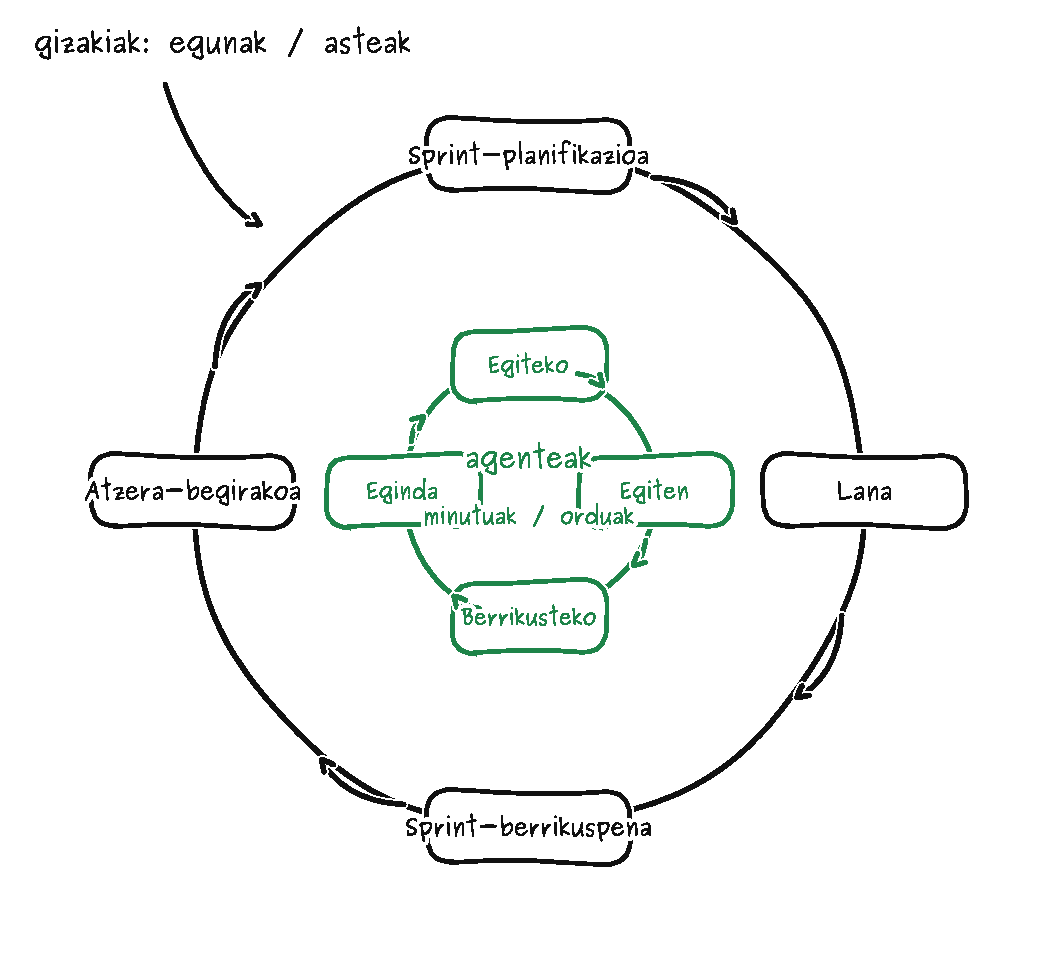
\includegraphics[width=0.8\textwidth]{Pictures/07/7.bi_begiztak.pdf}
    \caption{Scrumban agentikoaren bi erritmoak: \textit{Scrum}en begizta motela gizakientzat, eta \textit{Kanban}en begizta azkarra agenteentzat.}
    \label{fig:bi_begiztak}
\end{figure}

\section{Scrumban agentikoa, begirada batean}

\ref{tab:scrum_elementuak}~taulak laburbiltzen du \textit{Scrum}en elementu bakoitza zertan bihurtzen den Scrumban agentikoan.
Ia dena mantentzen da; aldatzen dena da nork egiten duen eta zer erritmotan.

\begin{table}[h]
    \centering
    \begin{tabular}{p{4cm}p{8.5cm}}
        \toprule
        \textbf{\textit{Scrum}en elementua} & \textbf{Scrumban agentikoan} \\
        \midrule
        Sprinta & Mantendu, gizakien erritmo gisa; ikasturteko mugarriekin lerrokatuta. \\
        Sprint-planifikazioa & Mantendu; zereginak agenteek egikaritzeko moduan idazten diren unea. \\
        \textit{Sprint backlog}a & Agenteek zereginak hartzen dituzten ilara, aldi berean lanean dagoen lanaren mugekin. \\
        Eguneroko \textit{Scrum}a & Scrumban-agentearen egoera-txostena gizakientzat. \\
        Egindakoaren definizioa & Integrazio jarraituaren eta berrikuspenaren ateak \textit{pull request} bakoitzean. \\
        \textit{Scrum} zuzendaria & Scrumban-agentea fluxuaren zaintzarako, eta gizakia taldearen prozesurako. \\
        Sprint-berrikuspena & Mantendu; gehikuntza interesdunei erakusten zaie, lehen bezala. \\
        Atzera-begirakoa & Mantendu; txantiloiak, zutabe-arauak eta ateak doitzen dira. \\
        \bottomrule
    \end{tabular}
    \caption{\textit{Scrum}en elementuak Scrumban agentikoan.}
    \label{tab:scrum_elementuak}
\end{table}

Lantaldeak lau rol ditu.
\textbf{Produktu-jabea} gizakia da, eta lehen bezala erabakitzen du zer eta zer ordenatan.
\textbf{Garatzaileak} gizakiak dira, baina haien lana aldatu egin da: kodea idatzi beharrean, zereginak idazten dituzte, agenteen lana berrikusten dute eta agenteak erabaki ezin duena erabakitzen dute.
\textbf{Scrumban-agentea} gainbegirale-agentea da: zereginak esleitzen ditu, agente langileen egoera-txostenak jasotzen ditu, blokeoak antzematen ditu, gizakiarengana eskalatzen du behar denean, eta lana ixten du ateak gainditutakoan.
\textbf{Agente langileak} kodetzeko agenteak dira, eta bakoitzak zeregin bakarra du esku artean: zeregin bat, adar bat, \textit{pull request} bat.

Lanaren unitatea \textbf{zeregina} da, \ref{cha:zereginak}.~kapituluan ikasi genuen moduan idatzia, eta proiektu-taulan bizi da, \ref{cha:taula}.~kapituluan eskuz kudeatu genuen moduan.
Zutabeak eta haien arauak dira metodoaren bihotza: Egiteko, Egiten, Berrikusteko eta Eginda, eta horiekin batera Blokeatuta eta gizakia behar duten zereginen zutabea.
Zutabe bakoitzak muga bat du eta arau idatziak, eta arau horiek dira agenteei ematen diegun jarraibide nagusia.

Hurrengo ataletan metodoaren mekanika zehaztuko dugu: zeregin baten egoera-makina, egoera batetik bestera nork eta noiz pasatzen duen; eskalatze-protokoloa, agenteak noiz eta nola eskatzen duen gizakiaren laguntza; eta trazabilitatea, zeregin batetik haren adarrera, \textit{pull request}era eta kodera iristeko bidea.

\section{Zereginaren egoera-makina}

\section{Eskalatze-protokoloa}

\section{Trazabilitatea: zereginetik kodera}
